% !TEX root = ../thesis-example.tex
%
\section{Persistence layer}
\label{sec:impr:persistence}

In this section we will discuss implementation of the Persistence layer of CHRYSALIS. We will list the problems solved by this tasks, details of the implementation both on the front- and backend side and results achieved by it. 

\subsection{Problem statement}
\label{sec:impr:persistence:problem}

Initially, when we got our hands on the project, CHRYSALIS stored all of the off-chain configuration data in the browser's local storage. Not only is it a safety concern (since the frontend user can easily manipulate data however they want), but also it is not reliable, since the browser's local storage could be cleaned on the user side and all of the data would be lost.\\

The other point of concern was that the only way to access deployed process model was by explicitly typing in its contract address, which renders the user interface completely useless and ruins user experience. Furthermore, to pick a task to execute, one had to explicitly specify the id assigned to it after the parsing into enzian model, which the user might not have even noticed. Lastly, there was no constraints on the task identifiers that could be chosen, so the user was perfectly capable of choosing an incorrect one and getting an error. To combat that, it was decided to implement a persistence layer, which would store all the off-chain information in a database, including information on associations between tasks and deployed processes. 

\begin{figure}[htb]
	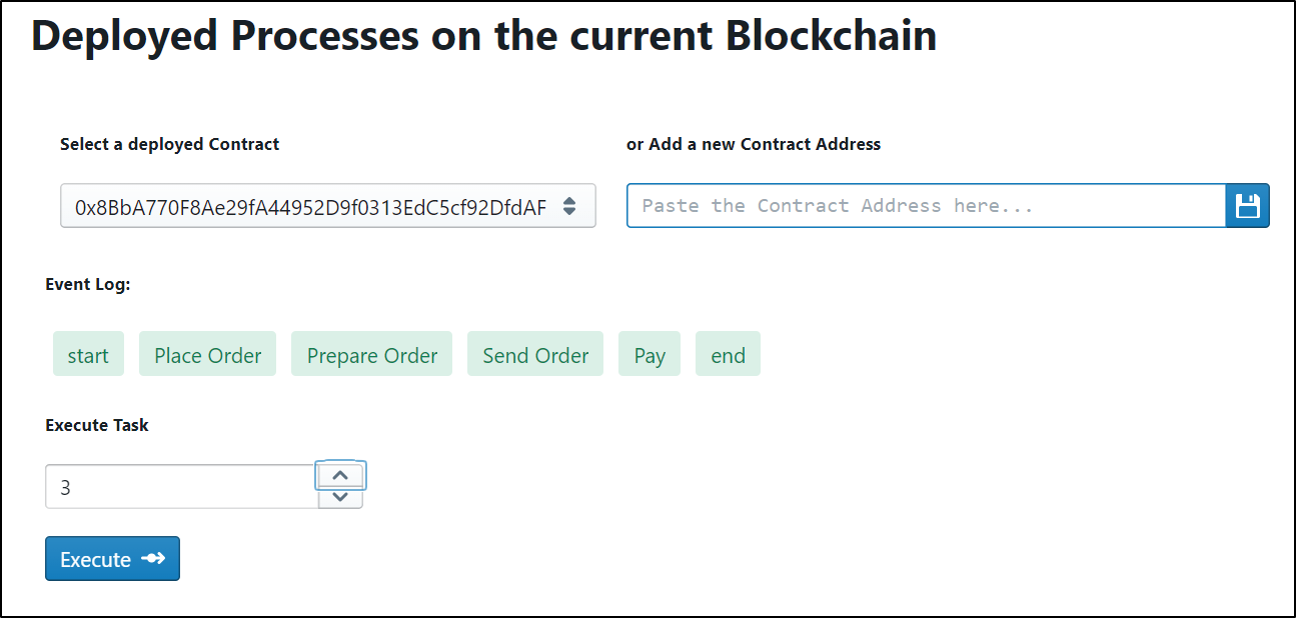
\includegraphics[width=\textwidth]{gfx/persistence_before}
	\caption{Process execution page before implementation of the persistence layer}
	\label{fig:impr:persistence:before}
\end{figure}

\subsection{Software stack}
\label{sec:impr:persistence:stack}

To implement this functionality it was decided to build a separate REST-server. For the server's implementation express.js framework was chosen, since the entire project is in javascript and express.js is meant for RESTful API implementation. PostgreSQL was chosen as a database management system, mainly because it is widely used and optimized for production, but free at the same time (unlike, for example, Oracle). It also provides a wide array of object-relational functionality, which could be useful further down the line in CHRYSALIS development. For exchange between the server and the database Sequelize ORM is used.

\begin{figure}[htb]
	\centering
	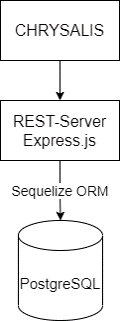
\includegraphics[width=.3\textwidth]{gfx/persistence_architecture}
	\caption{Persistence layer architecture}
	\label{fig:impr:persistence:architecture}
\end{figure}

\subsection{Backend}
\label{sec:impr:persistence:backend}

As is required by Sequelize ORM and express.js framework, the server code is divided into four packages: models, migrations, controllers and routes. Models contain a representation of database entities, including column datatypes, constraints, associations and cardinalities. Migrations contain scripts used for propagating the database schema created in the model package and all the changes made in that schema to the database. Every migration contains a function for propagating the changes and a function for undoing them. The controller package contains the server's business-logic, the database interactions in particular. The routes package provides REST-API endpoints for communication with the server.\\
 
The database schema is rather simple and consists of six entities (apart from the system ones, needed for the Sequelize ORM to work). Those entities are: Process, task, connection, abi, setting and account. The entities "Process" and "Task" are self-explanatory. Connections contain information about blockchain networks that the user could connect to. Account contains information regarding user's account on the blockchain network, such as their private key for signing transactions. Abi is an entity containing compiled smart contract code for executing a process model and is deployed every time a new process is uploaded to the system. The "Settings" entity contains current set of connection configurations, chosen by the user. Processes and Tasks are connected by a one-to-many association.

\begin{figure}[htb]
	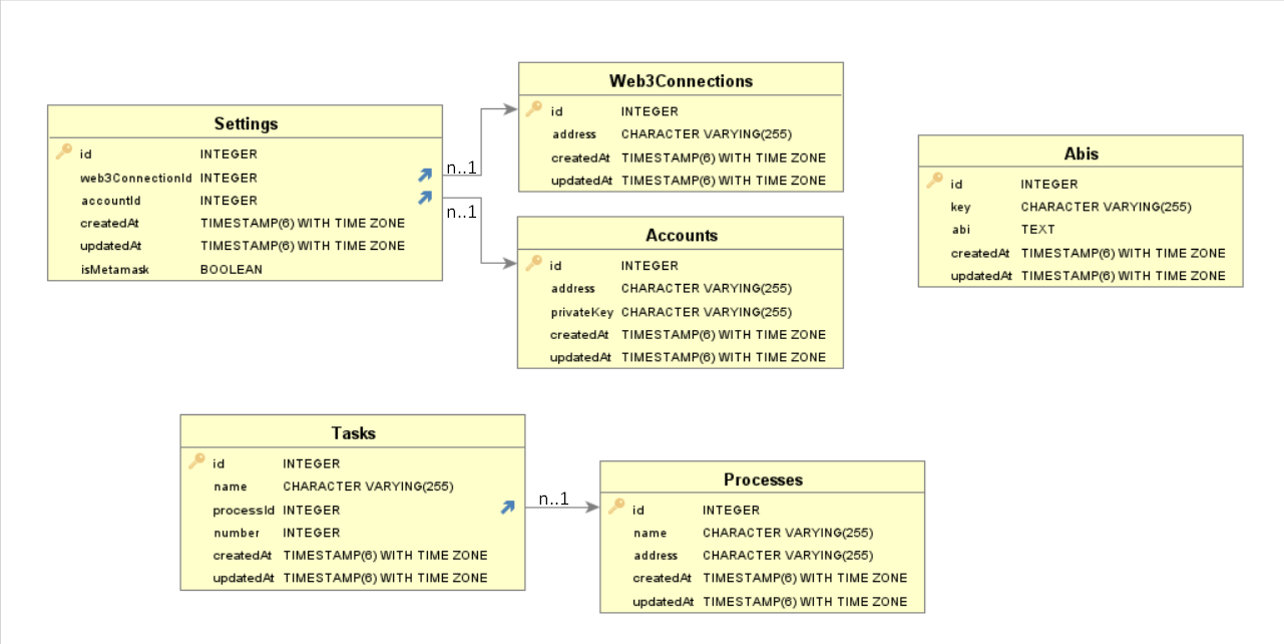
\includegraphics[width=\textwidth]{gfx/persistence_schema}
	\caption{Database schema}
	\label{fig:impr:persistence:schema}
\end{figure}

\subsection{Frontend}
\label{sec:impr:persistence:frontend}

On the frontend side we had to work within the confines of the existing application. The main means of RESTful exchange in react.js is Fetch-API. But the problem is that Fetch-API is very wordy and we would have to reuse large blocks lots of times, in every component of the application. Not only that, nut one would have to call this API with a wide array of different parameters, depending on the caller's intention. So it was decided to implement some universal exchange handling functionality within the frontend application.\\

To implement this it was decided to create an ExchangeHandler class which would be called by the application components to handle their requests. The components would pass to it the request method, URI and optionally data that they have to send, and then based on the method the exchange handler would find the appropriate instance of one of the sender classes and call them to execute the request. These sender classes are GetRequestSender, PostRequestSender, PatchRequestSender and DeleteRequestSender. They are instantiated and kept in the SenderRepository class. It contains a map with request methods as keys and sender instances as values. The exchange handler gets an appropriate sender from this map and calls its send() method to make a request to the server, returning a special promise objects, which provides methods to specify a logic, that should be executed once the response is received.


\begin{figure}[htb]
	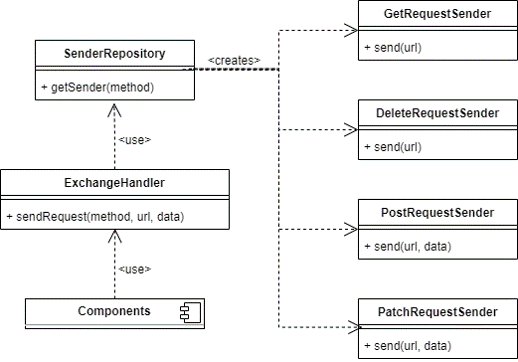
\includegraphics[width=\textwidth]{gfx/persistence_exchange}
	\caption{Database exhange module}
	\label{fig:impr:persistence:exchange}
\end{figure}

\subsection{Result}
\label{sec:impr:persistence:result}

After the changes made, all of the off-chain data was moved from the local storage to a separate database, improving safety and reliability. User experience was also significantly improved, since it became possible to choose deployed processes by their name from a list provided by the server, as well as choose from tasks associated with the process, by their name as well. The functionality of retrieving deployed processes by their contract addresses (if they are not present in the database) was preserved as well, but it underwent slight changes to make it compatible with the new architecture, and these changes will be discussed in the smart contract optimization section.

\begin{figure}[htb]
	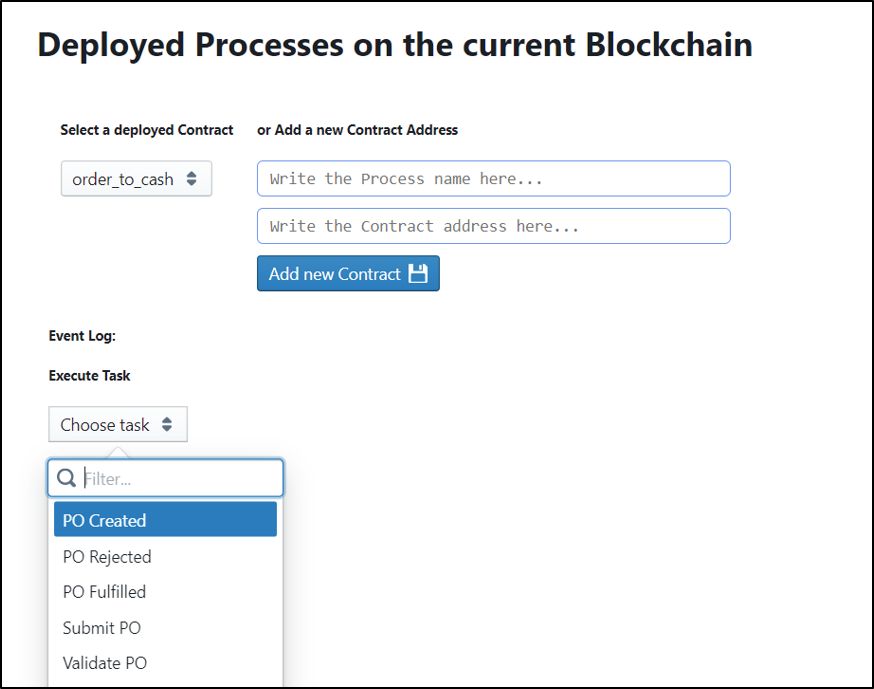
\includegraphics[width=\textwidth]{gfx/persistence_after}
	\caption{Process execution page after the improvements}
	\label{fig:impr:persistence:after}
\end{figure}


